\documentclass[a4paper]{article}
\usepackage[warn]{mathtext}
\usepackage[utf8]{inputenc}
\usepackage[T2A]{fontenc}
\usepackage[english,russian]{babel}
\usepackage{booktabs}
\usepackage{multicol}
\usepackage{fancyhdr}
\usepackage{graphicx}
\usepackage{microtype}
\usepackage{wrapfig}
\usepackage{amsmath}
\usepackage{floatflt}
\usepackage{geometry} \geometry{verbose,a4paper,tmargin=2cm,bmargin=2cm,lmargin=1.5cm,rmargin=1.5cm}
\usepackage{float}
\usepackage{amssymb}
\usepackage{caption}
\usepackage{epsfig}
\usepackage{newunicodechar}

\begin{document}

\graphicspath{ {pictures/} }
\begin{center}
    {\scshape\Large Лабораторная работа по твердотельной электронике} \par

    \

    {\huge\bfseries № 24: Полупроводниковый диод.} \par 

    \

    {\large Яромир Водзяновский Б04-852}
\end{center}

\

\
\textbf{Цель работы:} получение ВАХ полупроводникового диода, измерение емкости $p-n$ перехода, определенгие КРП.

\pagestyle{fancy} 
\fancyhead[L]{Твердотельная электроника   }
\fancyhead[R]{Лаборатораня работа}
\fancyhead[C]{}
\fancyfoot[C]{ \noindent\rule{\textwidth}{0.4pt} \thepage }



\section{Теоретическое описание}
\subsection{Образование переходной области}
Полупроводниковый диод (ПД) - прибор с нелинейной несимметричной вольт-амперной характеристикой (ВАХ) рис. 1.

\begin{figure}[h!]
    \centering
    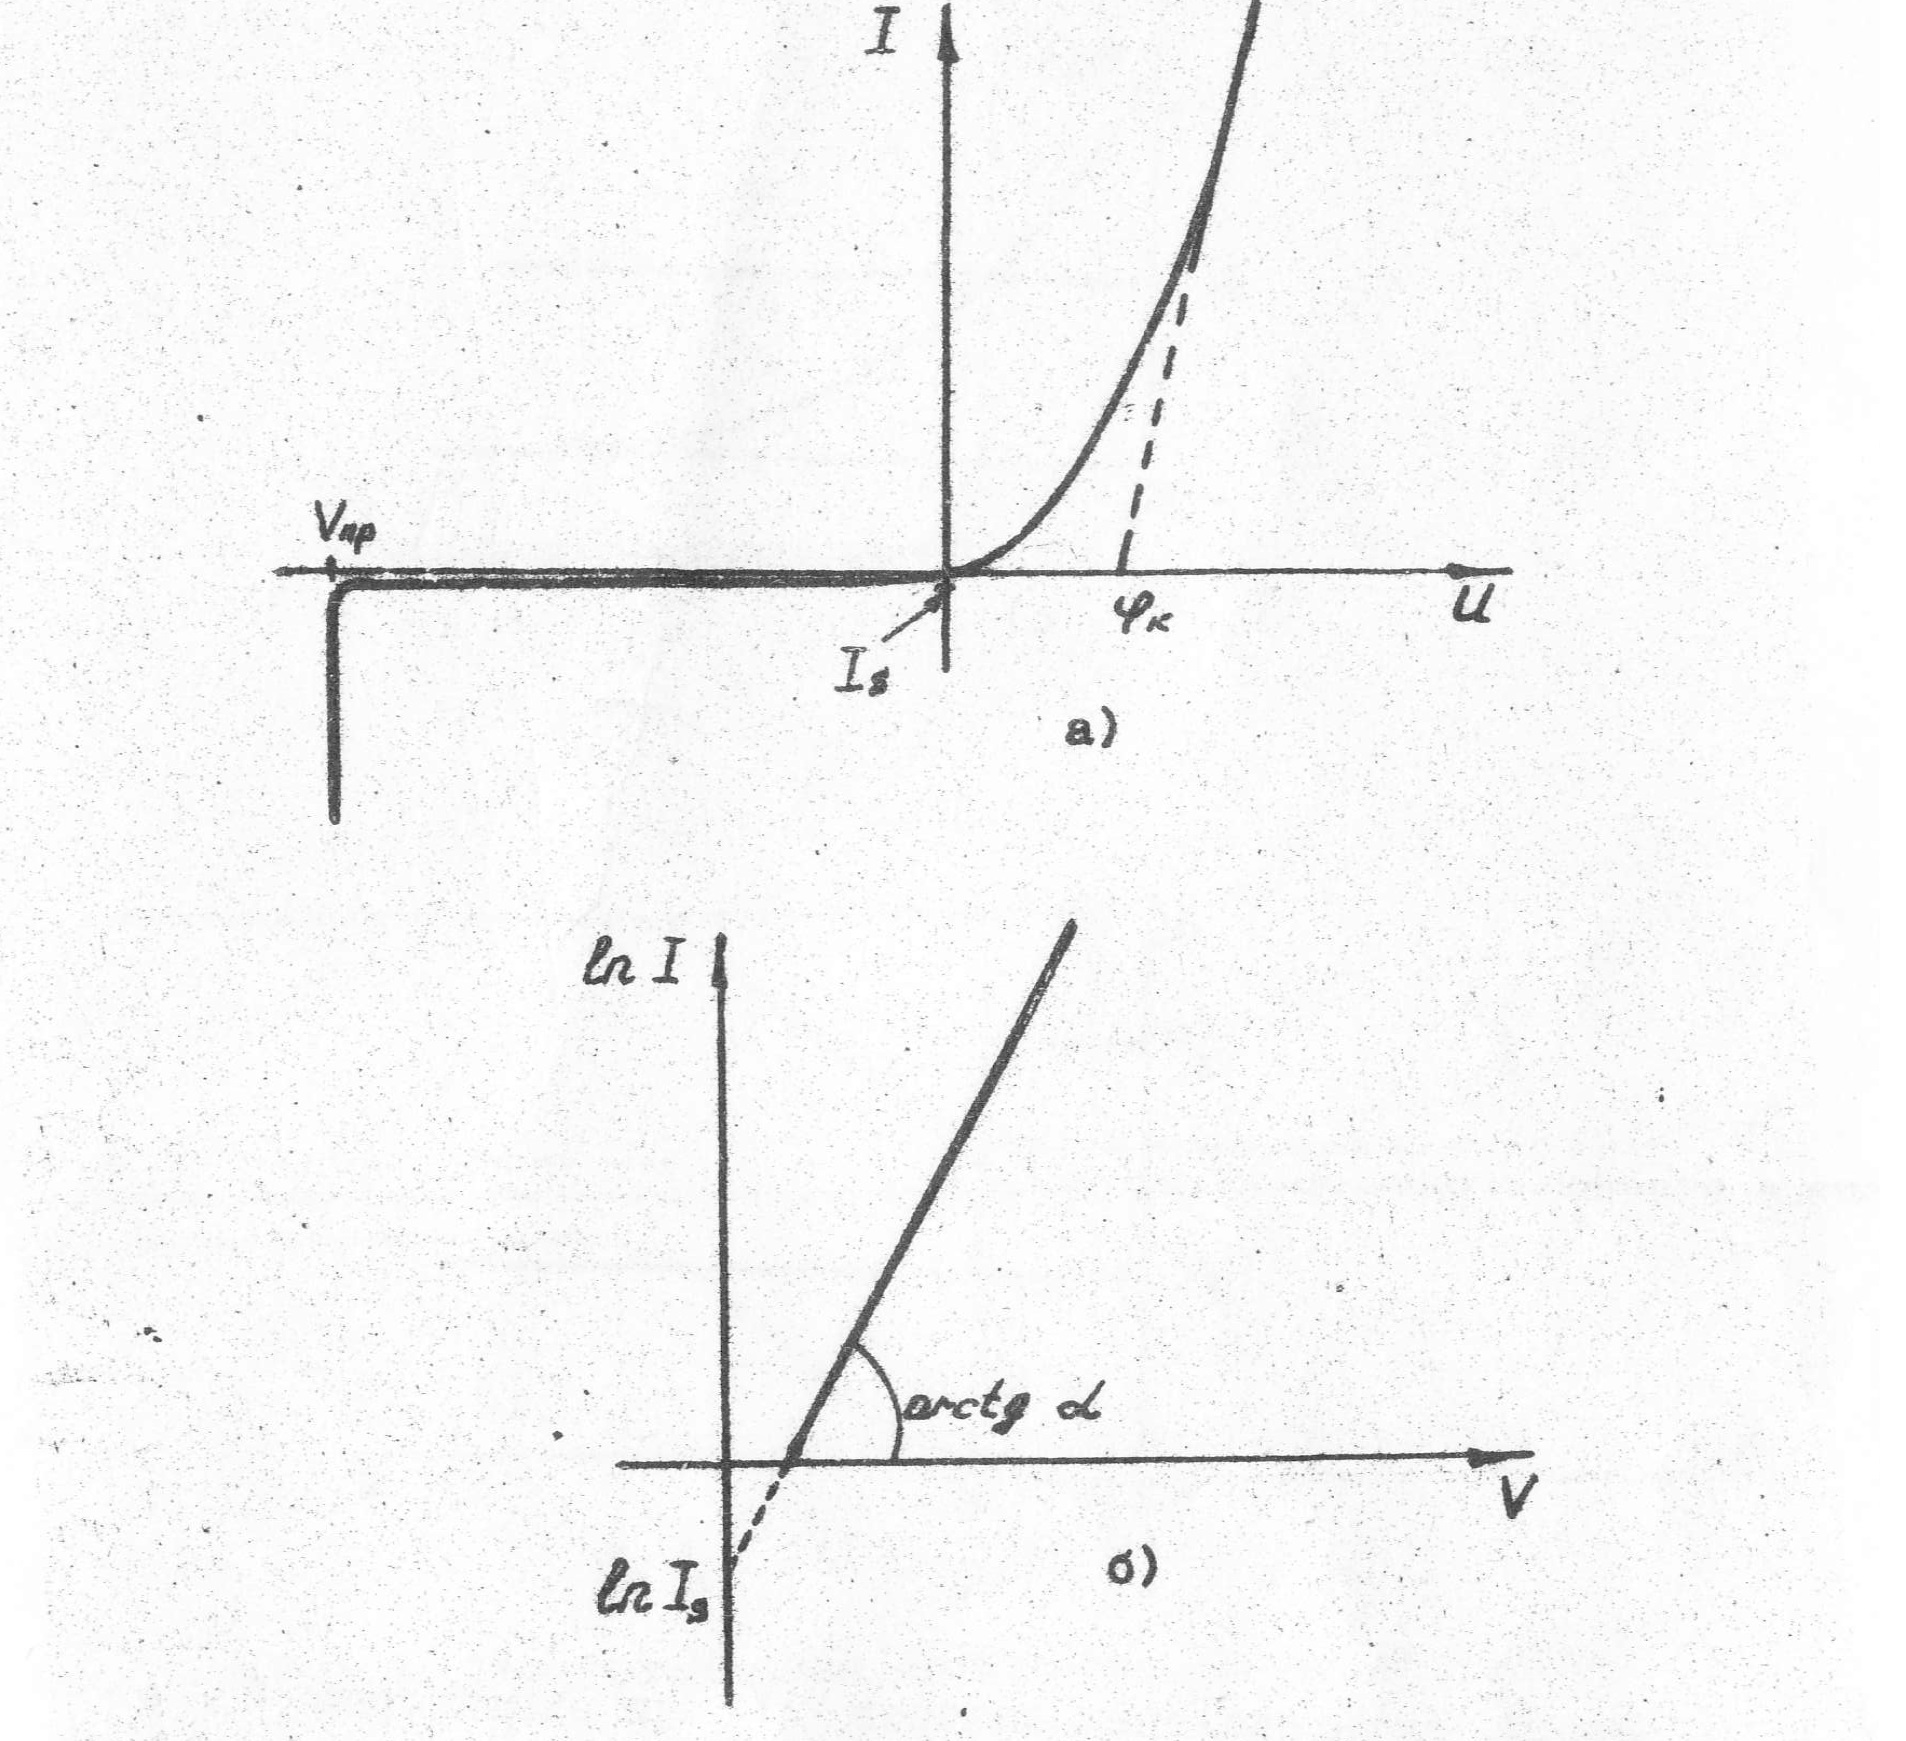
\includegraphics[scale=0.25]{VAH.jpg}
    \caption{ВАХ диода в полулогарифмическом (а) и логарифмическом(б) масштабе}
    \label{fig:VAH}
\end{figure}

Вид ВАХ ПД определяется свойствами потенциального барьера на границе, разделяющей области электронной (n - тип) и дырочной (p - тип) проводимости.

Рассмотрим образование барьера в резком p-n переходе. Пусть слева от $x = 0$ расположена p - область c концентрацией акцепторов (дырок) P, а справа - n - область с концентрацией доноров (электронов) N. Энергии ионизации лигирующих примесей таковы, что при рабочих температурах ПД все эти примеси ионизированы. Тогда
\begin{equation}
    p_p \approx P,
\end{equation}
    \begin{equation}
    n_n \approx N.
\end{equation}
В силу закона действующих масс в полупроводнике, в одной из областей (или в p - , или n - области)
\begin{equation}
    pn = n_i^2,
\end{equation}
где $n_i$ - собственная концентрация, тогда из (1)-(3) следует, что концентрация электронов и дырок равны соответственно
\begin{equation}
    n_p = \frac{n_i^2}{P},
\end{equation}
\begin{equation}
    p_n = \frac{n_i^2}{N},
\end{equation}
Из соотношений (1) - (5) видно, что при $N$ и $P$ серьёзно превышающих $n_i$ выполняются неравенства 
\begin{equation}
    n_n \gg  n_p,
\end{equation}
\begin{equation}
    p_p \gg p_p.
\end{equation}
Значит, через границу должны проходить диффузионные потоки электронов из n - области в р - область, а такде потоки дырок из p - облати в n - область. Но уходя из n - области электроны оставляют там нескомпенсированные положительно заряженные доноры, а дырки оставляют отрицательно заряженные акцепторы. Электрическое поле E нескомпенсированных зарядов препядствует переносу носителей заряда. В конечном итоге устанавливается диффузионно-дрейфовое равновесие, при котором диффузионные потоки компенсируют поле E (рис. 2).

\begin{figure}[h!]
    \centering
    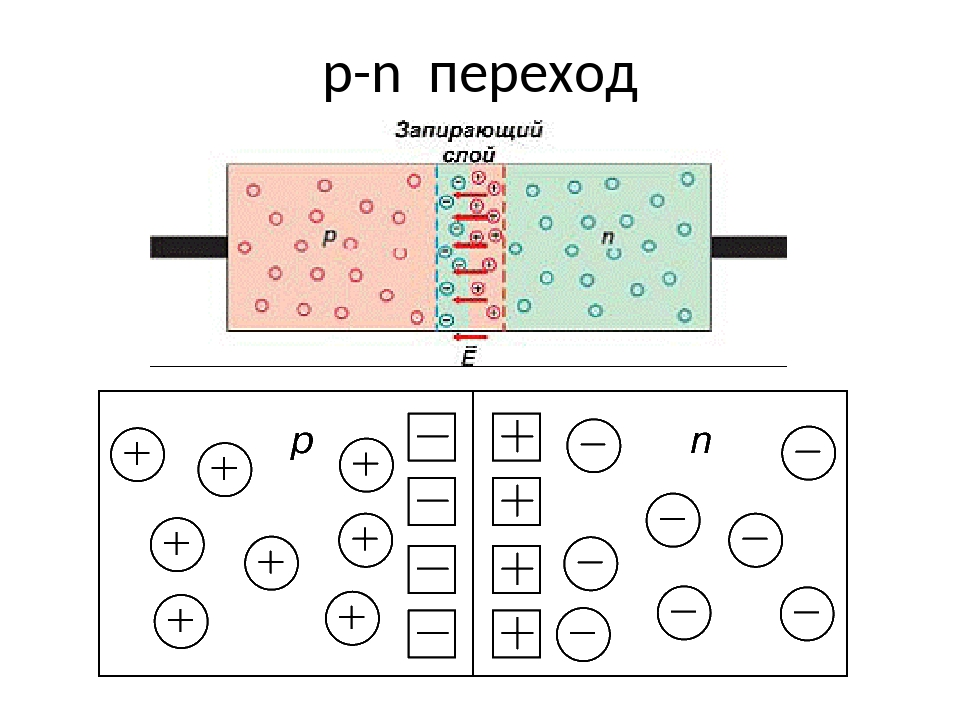
\includegraphics[scale=0.35]{image462.jpg}
    \caption{Распределение носителей заряда на границе p-n перехода}
    \label{fig:p-n}
\end{figure}

Наличие нескомпенсированных зарядов в переходной области приводит к появлению разности потенциалов между p - и  n - областями, называемой контактной разностью потенциалов. Возникает потенциальный барьер на границе этих двух областей с высотой $e\phi_{k}$, равный разности положений уровней ферми в изолированных полупроводниках p- и n- типа.
\subsection{Ширина переходной области}

    \begin{figure}[h!]
    \centering
    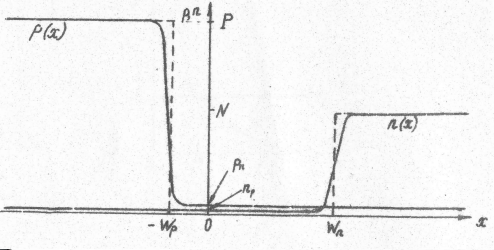
\includegraphics[scale=1]{im3.png}
    \caption{Распределение концентрации носителей в p-n переходе}
    \label{fig:concentrations}
\end{figure}

Из предыдущего раздела следует, что пространственное распределение концентраций электронов и дырок в p-n переходе (рис. 3) с хорошей точностью можно аппроксимировать соотношениями:
\begin{equation}
p(x) = \begin{cases} p_p, &  -\infty < x < -W_p \\ 0, & -W_p < x < \infty \end{cases}, \\
n(x) = \begin{cases} 0, &  -\infty < x < W_n \\ n_n, & W_n < x < \infty \end{cases}
\end{equation}
Из уравнения Пуассона, описывающего распределение потенциала имеем:
\begin{equation}
    \frac{d^2 \phi}{dx^2} = -\frac{4\pi e}{\varepsilon} \cdot \begin{cases}
    0, & -\infty < x < -W_p \\
    -P, & -W_p < x < 0 \\
    +N, & 0 < x < W_n \\
    0, & W_n < x < \infty \\
    \end{cases}
\end{equation}
Чтобы найти из (9) распределение  потенциала и размеры областей объёмного заряда $-W_p$, $W_n$ и $W = W_n + W_p$ необходимо задать граничные условия, получаемые из следующих соображений:
\begin{enumerate}
    \item вне области объёмного заряда поле равно 0,
    \begin{equation}
        \frac{d\phi}{dx}|_{x=-W_p}=\frac{d\phi}{dx}|_{x=W_n}=0,\\
    \end{equation}
    \item при $x=0$ $\phi$ и $E$ должны быть непрерывны, так как в противном случае на границе возникли бы бесконечные поле и плотность объёмного заряда,
    \begin{equation}
        \frac{d\phi}{dx}|_{x=0-0}=\frac{d\phi}{dx}|_{x=0+0}, \phi(0-0) = \phi(0+0), \\
    \end{equation}
    \item при том условии, что при $x=W_n$ потециал принят за 0, при $x=-W_p$ потенциал равен $-\phi_k$.
    \begin{equation}
        \phi(-W_p)=-\phi_k, \phi(W_n) = 0.
    \end{equation}
    \end{enumerate}
    Из (9)-(12) получаем:
    \begin{equation}
    W = \sqrt{\frac{\varepsilon \phi_k}{2\pi e}(\frac{1}{N}+\frac{1}{P})},
    \end{equation}
    причем
    \begin{equation}
        PW_p=NW_n
    \end{equation}
    В несимметричном случае, когда, например, $P \gg N$ $W \approx W_n$.
    
    При прикладывании напряжения V высота барьера меняется на eV, равновесие в переходе нарушается, однако, если это нарушение невелико, то можно считать, что носители по прежнему имеют больцмановское распределение, и тогда 
    \begin{equation}
    W = \sqrt{\frac{\varepsilon (\phi_k - V)}{2\pi e}(\frac{1}{N}+\frac{1}{P})},
    \end{equation}
    \subsection{ВАХ p-n перехода}
    Для нахождения связи между концентрациями электронов и дырок слева и справа от p-n перехода сделаем замену, аналогичную прошлому пункту:
    \begin{equation}
        p(W_n) = p_n(\exp{\frac{eV}{kT}}), n(-W_p) = n_p(\exp{\frac{eV}{kT}})
    \end{equation}
    Плотность тока диффузии носителей описывается следущим образом:
    \begin{equation}
        j_p = -e D_p \frac{dp}{dt}, W_n < x, \\
        j_n = e D_n \frac{dn}{dt}, x < -W_p.
    \end{equation}
    Здесь $D_p$ и $D_n$ - коэффиценты диффузии дырок и электронов. При малых уровнях инжекции дрейфовыми состовляющими плотностей токов можно пренебречь. Вглубине P- и n- областей носители рекомбинируют со скоростями
    \begin{equation}
        v=\frac{p-p_n}{\tau_p}, v=\frac{n-n_p}{\tau_n}
    \end{equation}
    Здесь $\tau_p$ и $\tau_n$ - времена жизни дырок и электронов. Также из уравнений непрерывности:
    \begin{equation}
        \frac{dj_p}{dx} = -e\frac{p-p_n}{\tau_p},
        \frac{dj_n}{dx} = e \frac{n-n_p}{\tau_n}.
    \end{equation}
    Решая совместно (16) и (18) получим ВАХ вида:
    \begin{equation}
        I=I_s(\exp{\frac{eV}{kT}}-1),
    \end{equation}
    где $I_s = S(\frac{eD_pp_n}{L_p}+\frac{eD_nn_p}{L_n})$, $L_p = \sqrt{D_p\tau_p}$, $L_n = \sqrt{D_n\tau_n}$.
    ВАХ реальных ПД серьёзно отличаются от полученной. Есть несколько основных отличий:
    \begin{enumerate}
        \item При $U>\phi_k$ ВАХ линейна и имеет вид $I=(U-\phi_k)/r_b$.
        \item При $U<\phi_k$ ВАХ имеет вид
        $I=I_s(\exp{\frac{eV}{\nu kT}}-1)$, $1<=\nu<=2$
        \item Обратная ветвь ВАХ реальных ПД почти не имеет насыщения
        \item Имеется пробой при больших обратных напряжениях.
    \end{enumerate}
    Рассмотрим причины возникновения особенностей:
    1) 	При расчете ВАХ предполагалось, что все внешнее напряжение приложено к барьеру. Однако в действительности часть внешнего напряжения падает не на барьере, а на нейтральных p- и n- областях и ВАХ должна иметь вид:
    \begin{equation}
        I=I_s [\exp{\frac{e (U-I r_b)}{kT}} - 1].
    \end{equation},
    где $r_b$ - сопротивление нейтральных p-n областей. Падение напряжения на барьере не может превысить $\phi_{k}$, а значит при приложенных напряжениях $U-Ir_b \sim \phi_{k}$ рост внешнего напряжения приводит к росту $Ir_b$, что и даёт переход из экспоненциальной зависимости в линейную.
    
    2) и 3) возникают из-за наличия токов рекомбинации, которыми мы пренебрегли при поиске вида ВАХ. Такое пренебрежение оказывается не всегда справедливо, что и приводит к возникновению коэффицента $\nu$. Таким образом, полный ток через p-n переход будет равен:
    
    \begin{equation}
        I = I_s (\exp{\frac{eU}{kT}} - 1) + I_{pns} (\exp{\frac{eU}{\nu kT}} - 1)
    \end{equation}
    
    4) Пробой возникает по нескольким причинам. Тепловой пробой легко устранить при хорошем теплоотводе от диода. Лавинный пробой обусловлентем, что при больших прикладываемых напряжениях носители приобретают энергию достаточную для ионизации решетки. Этот пробой происходит лавинообразно. Приближенный вид зависимости $V_{np}(N)$:
    \begin{equation}
        V_{np} \sim \frac{{E_{np}}^2}{N} \sim \rho
    \end{equation}
    Также при больших напряжениях расстояние между электронами в валентной зоне и свободными уровнями может стать сравнимой с волной де Бройля электронов. При возникновении подобной ситуации появляется возможность туннелирования в зону проводимости электронов, что также ведет к нарастанию тока. Если принять, что интенсивное туннелирование начинается при $\Delta x = \Delta x_{kp} $, то:
    \begin{equation}
        V_{np} \sim \frac{1}{N} \sim \rho
    \end{equation}
    Точный расчет дает именно такую зависимость.
    
    \subsection{Ёмкость запорного p-n перехода}
    Электронно-дырочный переход представляет собой обедненную подвижными носителями область полупроводника, близкую по своим свойствам к слою диэлектрика, в котором по разные стороны от некоторой плоскости находятся объемно распределенные неподвижные электрические заряды противоположных знаков. В этом смымле p-n переход ведет себя как ёмкость.
    
    
    
    Найдём ёмкость перехода из статических соображений. При изменении заряда на dQ:
    \begin{equation}
        dQ = eNSdW_n = ePSdW_p = Cd(\phi_k-V).
    \end{equation}
    Используя (13) получим
    \begin{equation}
        C=S\sqrt{\frac{\varepsilon N P}{8\pi e(N+P)(\phi_k-V)}}
    \end{equation}
    При N << P
    \begin{equation}
        C=S\sqrt{\frac{\varepsilon N}{8\pi e N(\phi_k-V)}}
    \end{equation}
    Зависимость ёмкости запорного перехода от приложенного напряжения можно увидеть на рисунке \ref{fig:Condecer}. Вместо дальнейшего выписывания математических выкладок увидим из графика, что С можно представить как
            \begin{equation}
        C=\frac{\varepsilon S}{4\pi W}
    \end{equation}
    
    \begin{figure}[h!]
    \centering
    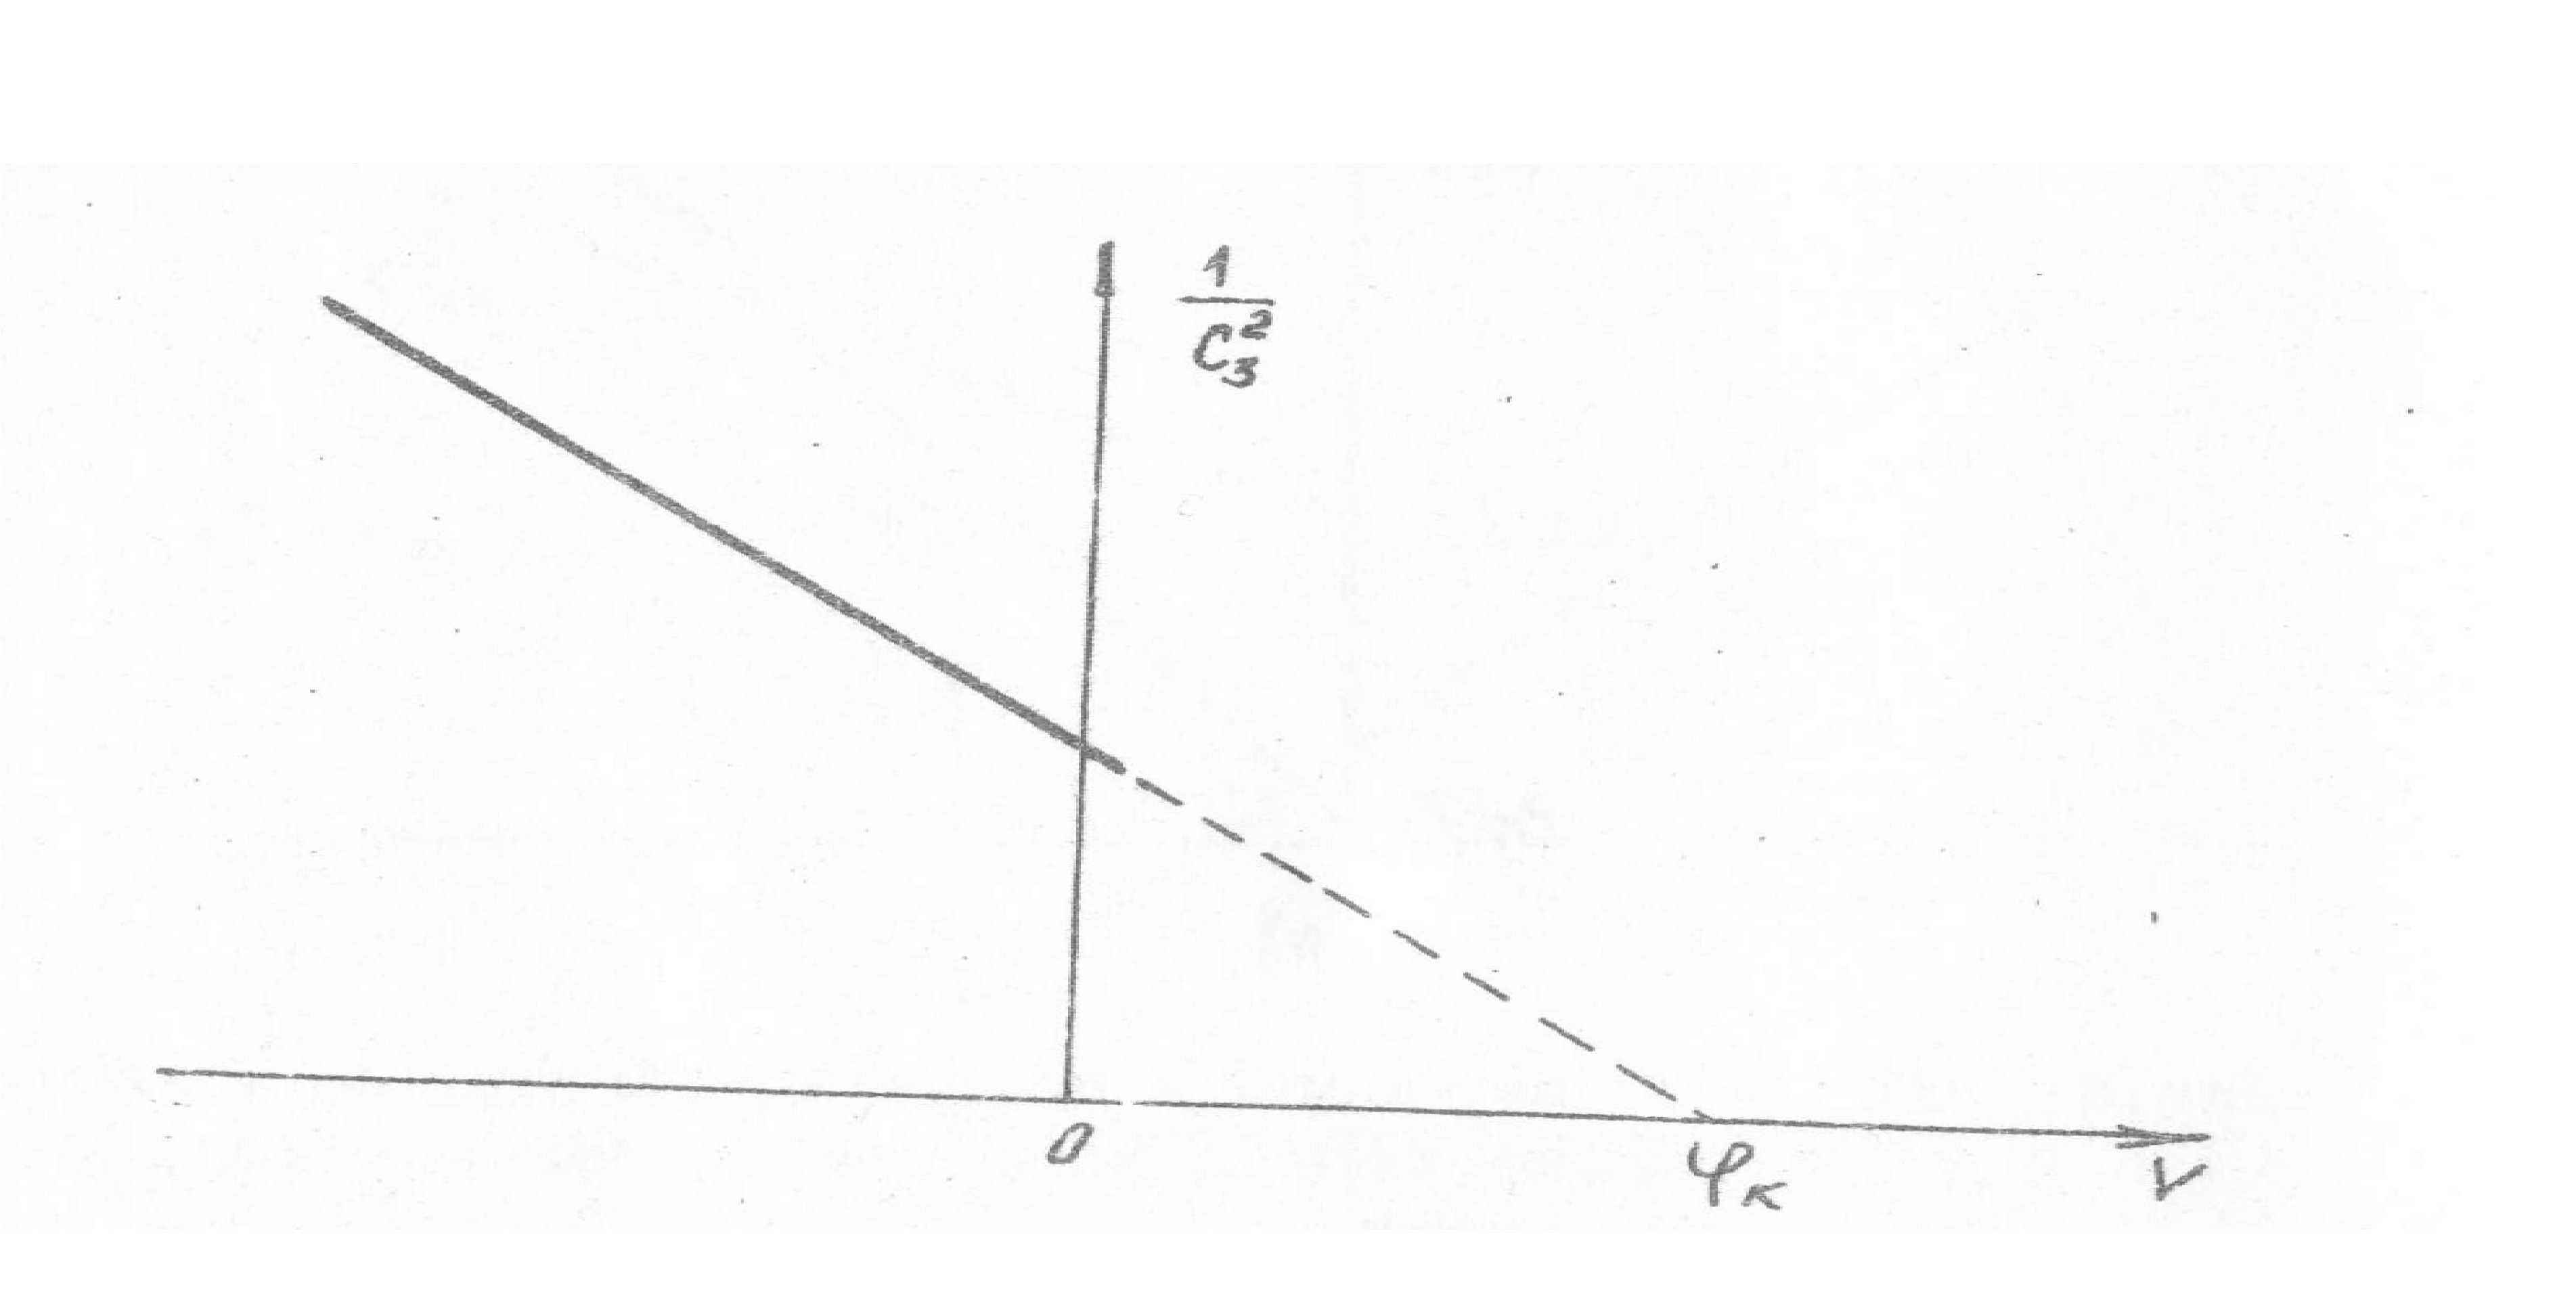
\includegraphics[scale=0.13]{Condecer.jpg}
    \caption{Зависимость $\frac{1}{С^2}$ от V}
    \label{fig:Condecer}
\end{figure}
    
\section{Описание измерительной установки}
Принципиальная схема установки приведена на рисунке (\ref{fig:Scheme}):

\begin{figure}[H]
    \begin{center}
    \center{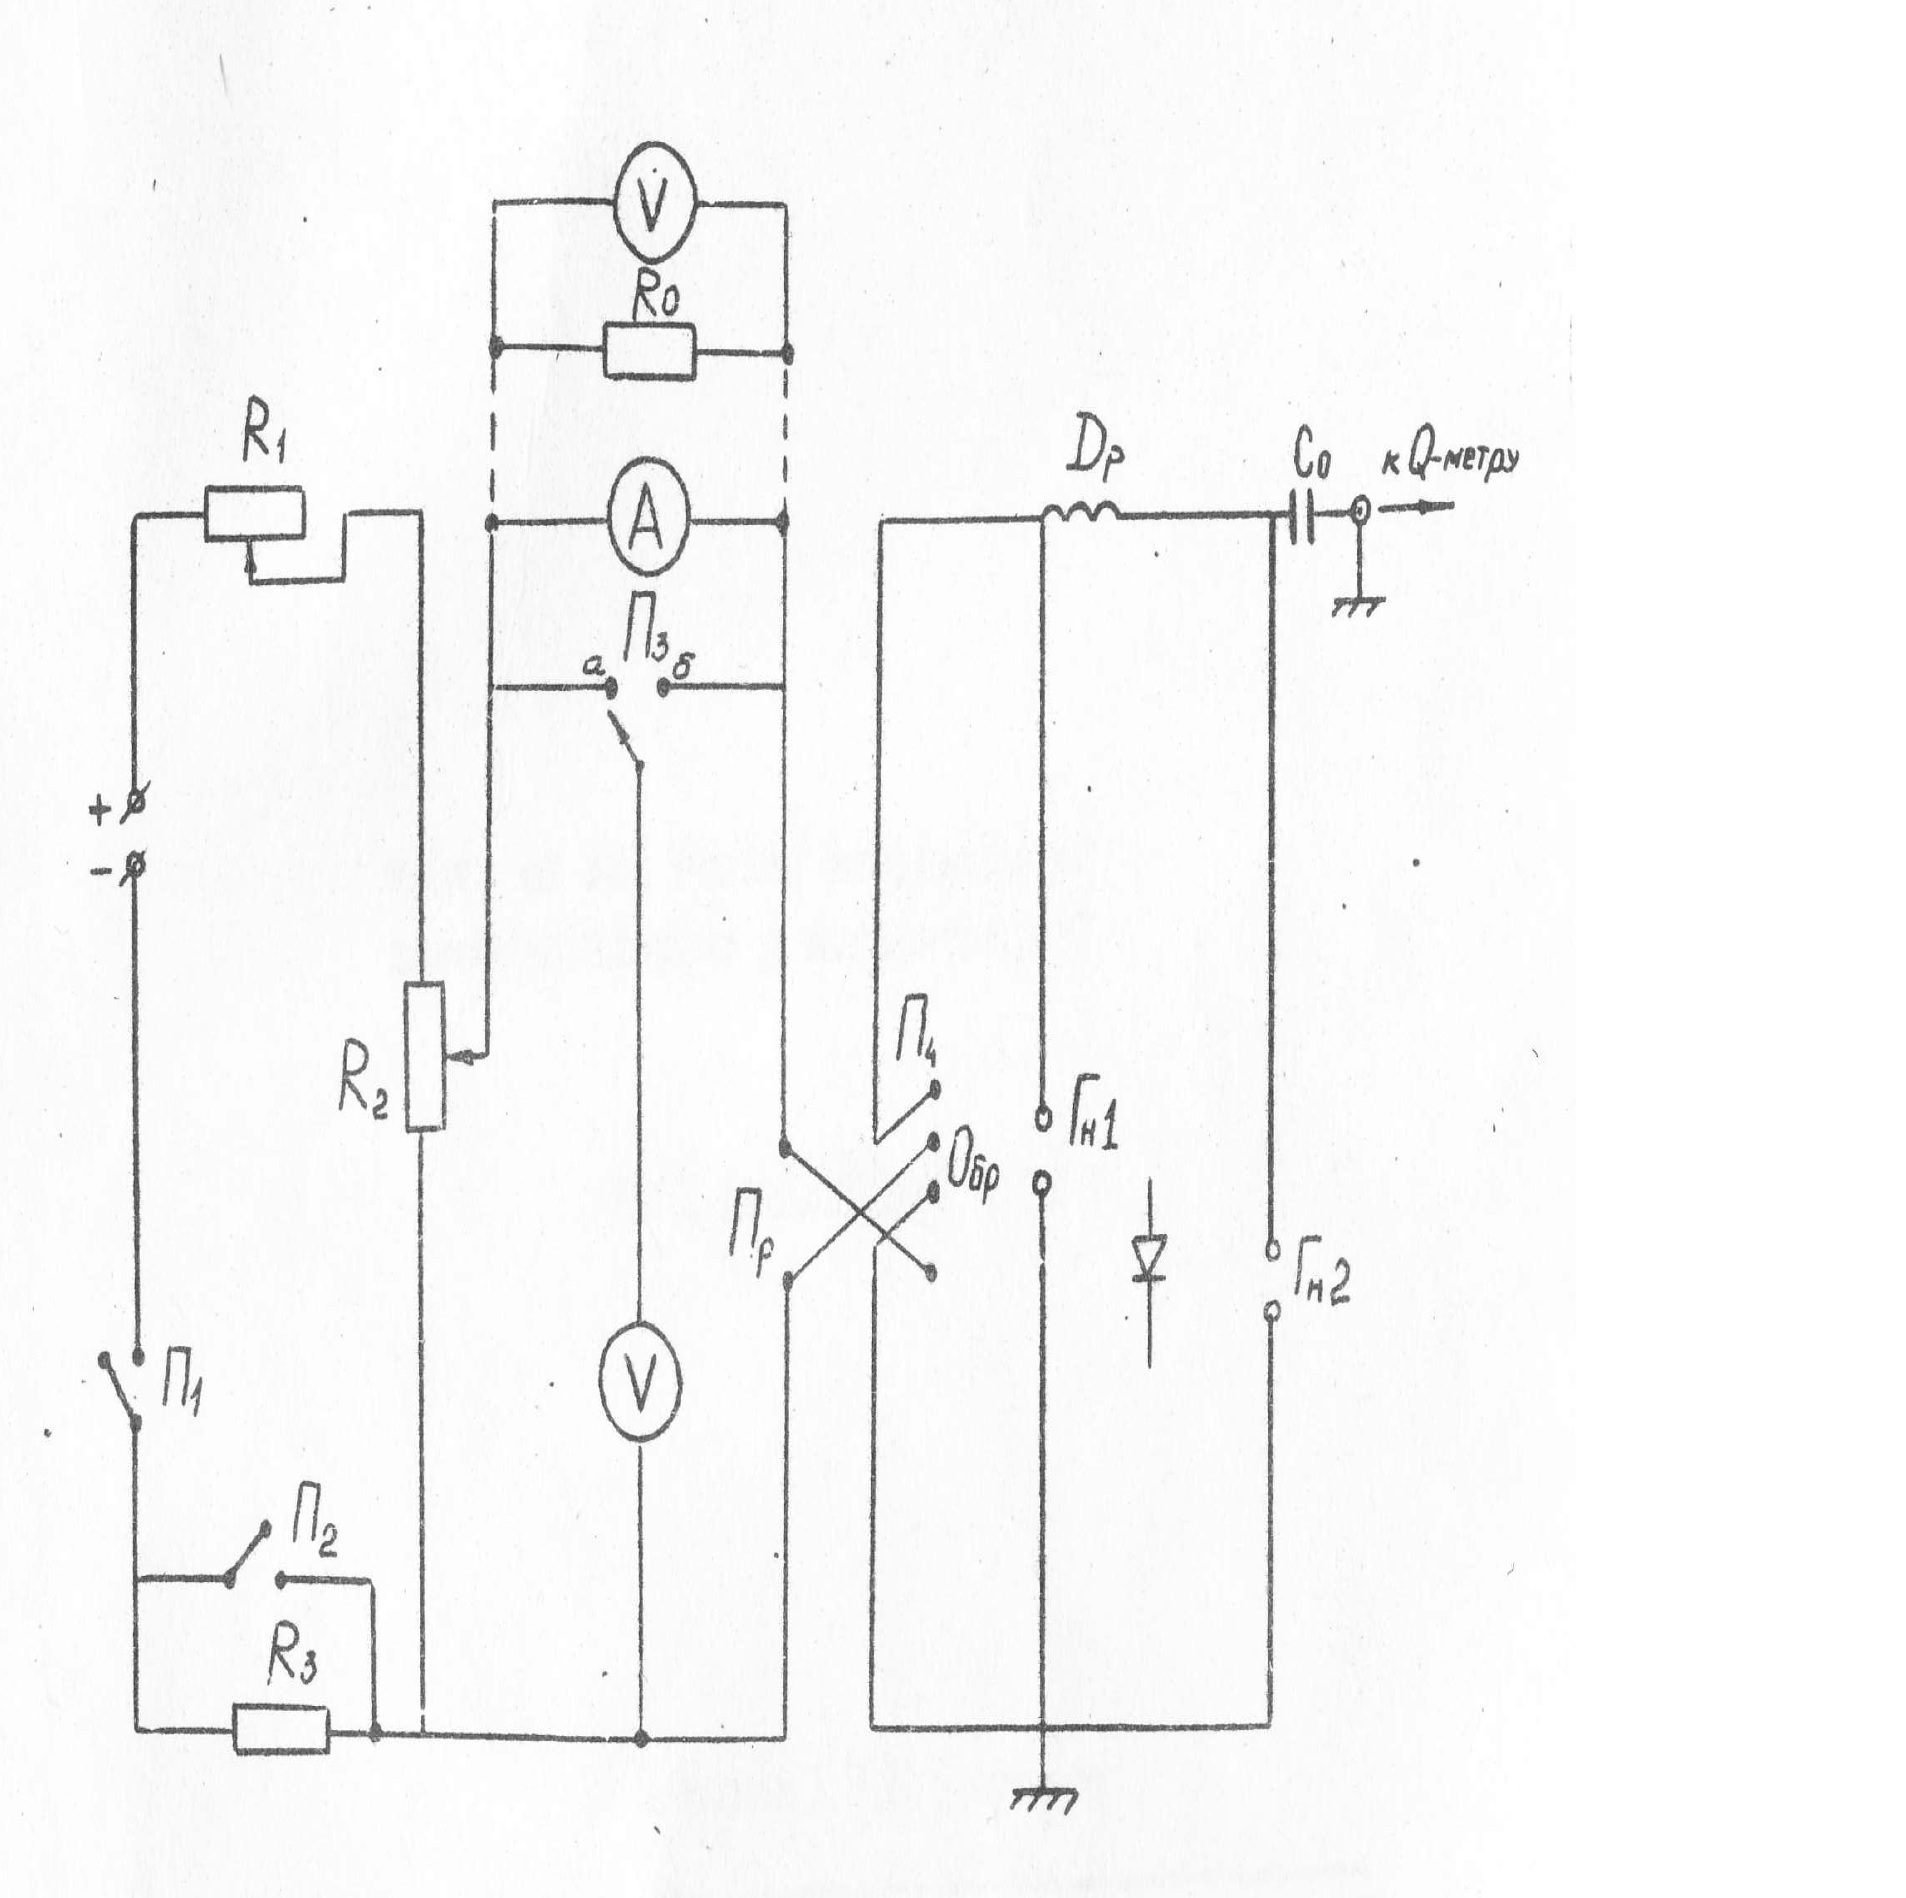
\includegraphics[scale=0.2]{Diode_Scheme.jpg}}
    \caption{Принципиальная схема измерительной установки}
    \label{fig:Scheme}
    \end{center}
\end{figure}


При снятии прямой ветви ВАХ диода напряжение на диод подается с делителя, образованного из $R_1$, $R_3$ и потенциометра $R_2$. Регулируя сопротивления $R_1$ и $R_2$ можно можно изменять напряжение на диоде. При снятии обратной ветви резистор $R_3$ закорачивается и пределы измерения напряжения увеличиваются.

Измерения тока производятся либо с помощью стрелочного микроамперметра, либо с помощью вольтметра, контролирующего напряжение на $R_0$.

При престанове диода для изменения ёмкости дроссель позволяет снизить величину паразитной ёмкости схемы и отделяет диод от Q-метра по постоянному току.

Измерения ёмкости производится с помощью Q-метра следующим образом. Без диода контур Q-метра настраивают на резонанс посредством изменения ёмкости контура. Полученная ёмкость контура фиксируется. При подключении в цепь диода в контуре снова изменяется ёмкость до достижения резонанса. Разность между изначальной и новой ёмкостью будет равен барьерной ёмкости. 
\section{Методы получения величин}
Построение ВАХ и С(V) описаны выше в разделе "Описание измерительной установки".

Если построить ВАХ в логарифмическом масштабе угол наклона прямой ВАХ будет равен $\frac{e}{kT} = \frac{1}{\phi_T}$.

Из ВАХ угла наклона ВАХ можно найти сопротивление базы - оно обратно пропорционально углу наклона линейного участка прямой ветви. Если проэкстарполировать линейный участок до оси напряжений, то точка пересечения проэкстарполированной прямой с горизонтальной осью равен контактной разности потенциалов.

После построения зависимости $\frac{1}{C^2}$ от обратного напряжения N легко находится из наклона зависимости при том условии, что известна S. $\phi_{k}$ находится путем экстраполирования линейной зависимости до оси X. 

\section{Дополнительный вопрос}
\textit{Как с «физической» точки зрения объяснить тот факт, что на прямой ветви полупроводникового диода после подаваемого напряжения, превышающего контактную разность потенциалов, экспоненциальный ход зависимости переходит в линейный?}\\


Мы прикладываем напряжение, сначала ВАХ имеет экспоненциальный характер, т.к концентрация носителей описывается распределением Ферми-Дирака, однако в нашем случае оно Больцмановское ($\Delta \gg kT$). \par 
Начиная с некоторого значения напряжения $U_{пр}$, характеристика становится почти линейной, т.к. запирающий слой почти исчезает на линейнойм участке сопротивление диода обусловлено почти постоянным сопротивлением $p-$ и $n-$областей.
\begin{figure}[h!]
    \centering
    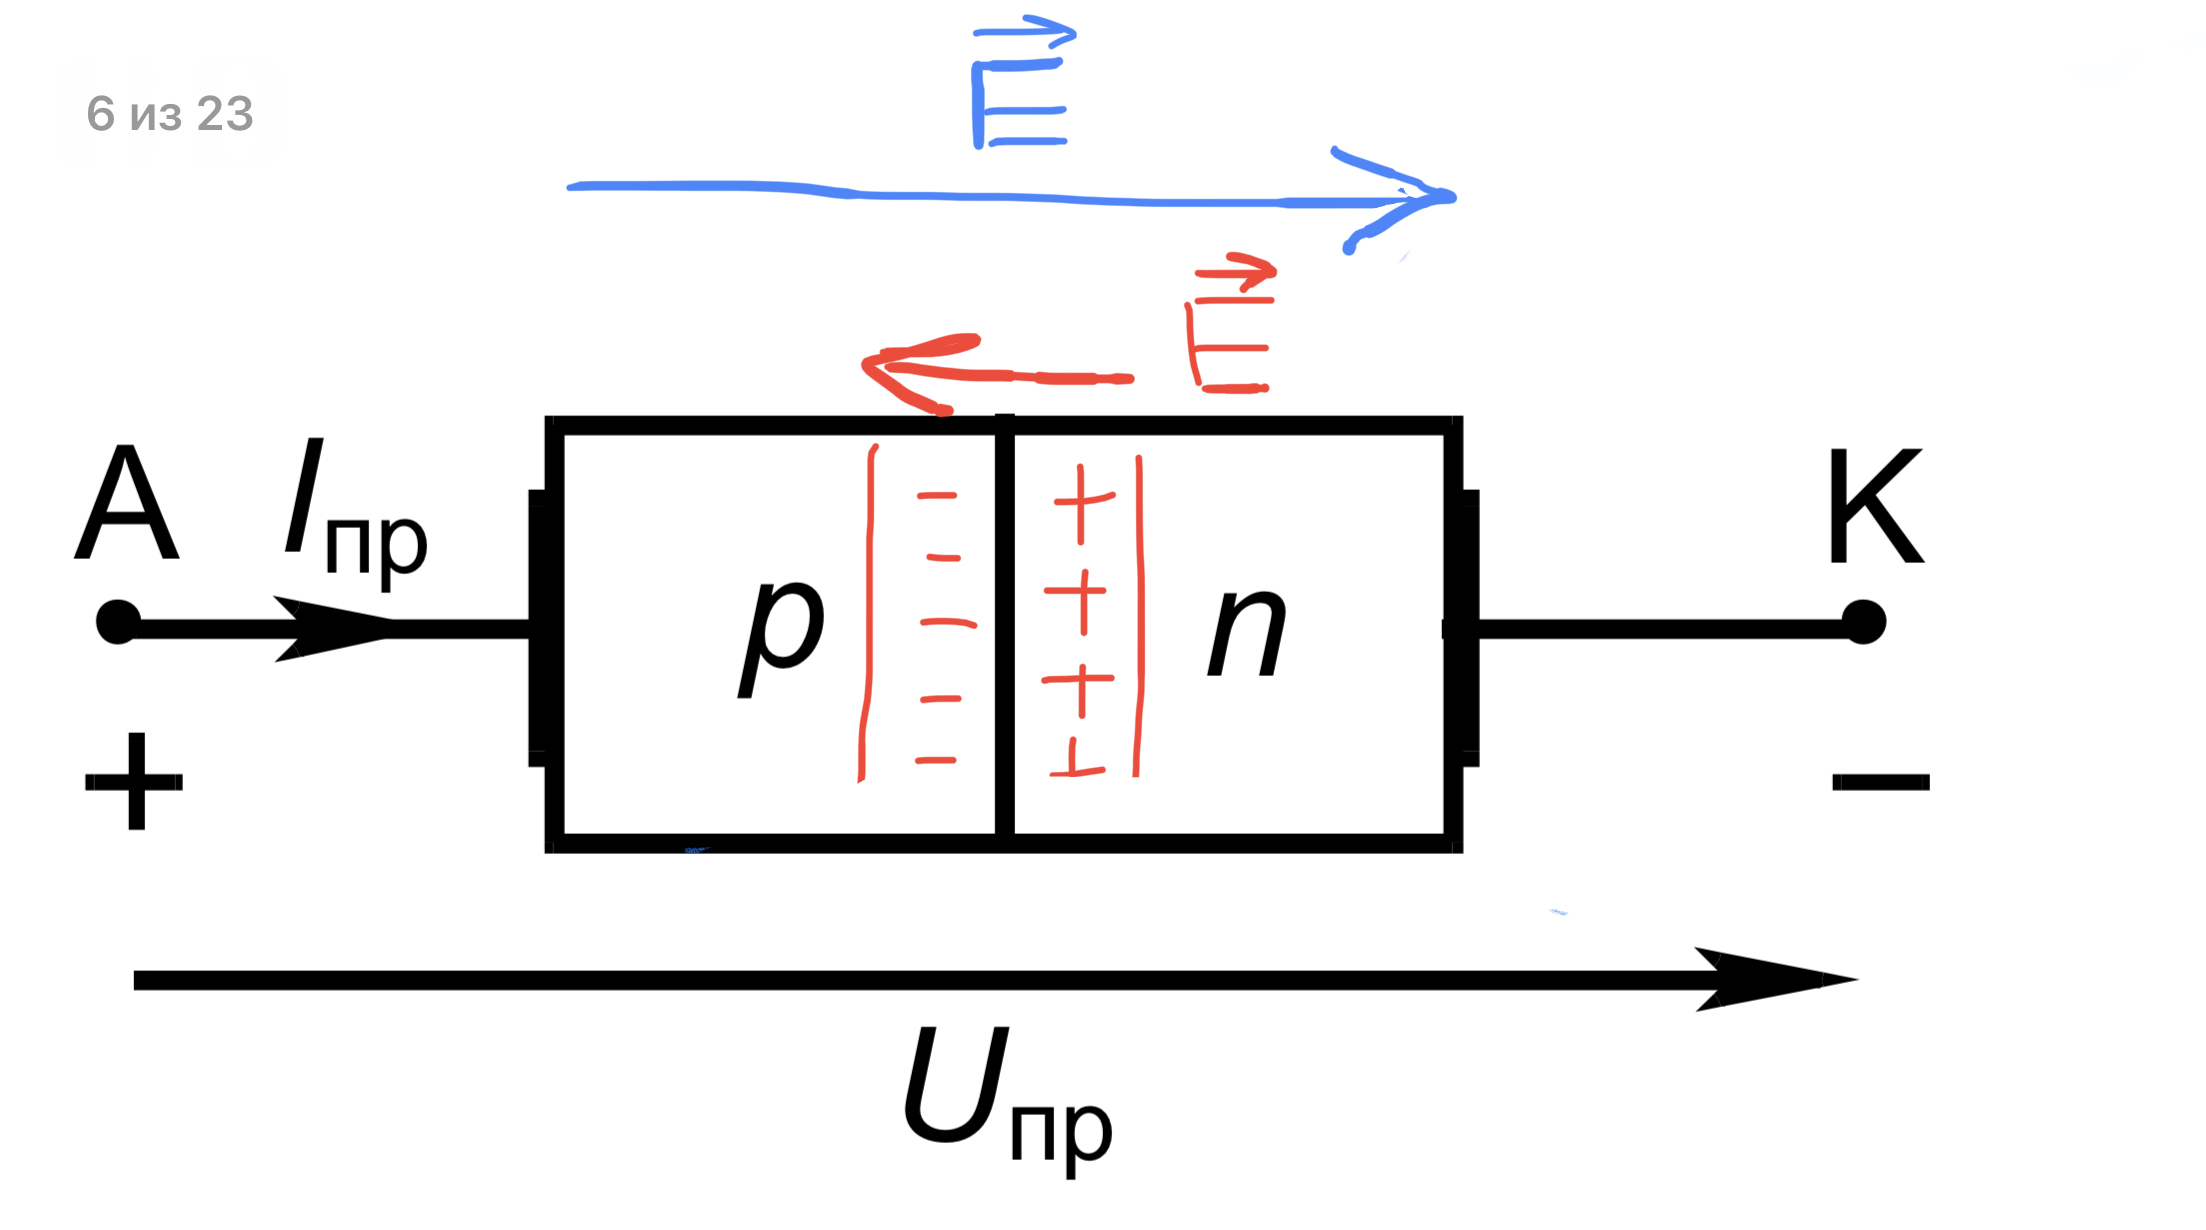
\includegraphics[scale=0.2]{IMG_3733.jpg}
    \caption{Схема р-n перехода}
    \label{fig:quest}
\end{figure}

\end{document}














